\chapter{Evaluation}
\label{sec:evaluation}

% Zu jeder Arbeit in unserem Bereich gehört eine Leistungsbewertung. Aus
% diesem Kapitel sollte hervorgehen, welche Methoden angewandt worden,
% die Leistungsfähigkeit zu bewerten und welche Ergebnisse dabei erzielt
% wurden. Wichtig ist es, dem Leser nicht nur ein paar Zahlen
% hinzustellen, sondern auch eine Diskussion der Ergebnisse
% vorzunehmen. Es wird empfohlen zunächst die eigenen Erwartungen
% bezüglich der Ergebnisse zu erläutern und anschließend eventuell
% festgestellte Abweichungen zu erklären.

% Checked
This chapter evaluates the implementation of the developed
system with respect to performance and flexibility.  The
evaluation has emphasis on determining the overhead of CAL and GVON
configured with the MPI adapter in comparison to plain MPI.

It is expected that the overhead is negligible, because of
compile-time optimization. Therefore, there will be no difference if
MPI is exchanged by the GVON. Such that, communication processes will
be as fast as the underlying adapter implementation.

The evaluation is divided in several benchmarks and every benchmark
provides several experiments. Synthetic benchmarks will evaluate
single communication methods. Instead, real world benchmarks
will compare the implemented simulations in comparison to equivalent
MPI implementations. Finally, the flexibility benchmark evaluates the
behavior of the system when vertices are redistributed at run-time.
Thereby will experiments vary in amount of hosts, number of messages
to send, number of elements to send, and usage of network.

The benchmark system is the HPC system of the Helmholz
Zentrum Dresden Rossendorf (HZDR)\cite{ref:hzdr_cluster}.
%% and the
%% system of the Zentrum für Informationsdienste und Hochleistungsrechnen
%% (ZIH).
A part of the HZDR system is the hypnos linux cluster (Ubuntu 12.04.4
LTS) consisting of two head nodes and more than 150 compute nodes.
The so-called laser nodes combine 4 AMD Interlagos Opterons by 4
sockets on a single mainboard resulting in 64 CPUs per node.  The
Interlagos Opterons 6276 are two Valencia chips on a single die,
whereby 2 core share a 64 KB L1 Cache and a 2 MB L2 Cache. Laser nodes
are interconnected by an Infiniband network. These nodes are utilized
for all synthetic, real simulation, and flexibility benchmarks.

%% In turn, are
%% kepler nodes equipped with 2 Quad-Core Xeon CPUs from Intel clocked by
%% 2,4 GHz. These nodes are used if only a pair of peers is necessary for
%% a benchmark.

%% The ZIH system provides a cluster called taurus. The nodes are
%% equipped each with two Intel Xeon(R) CPU : sandy E5-2690 (8 cores),
%% gpu E5-2450 (cores), west X5660 (6 cores).

The nodes provide their software environment by the module system.
The software is compiled by g++ 4.8.2 with OpenMPI 1.8.0.

%%%%%%%%%%%%%%%%%%%%%%%%%%%%%%%%%%%%%%%%%%%%%%%%%%%%%%%%%%%%%%%%%%%%%%%%%%%%%%%%
%                                                                              %
% SYNTHETIC POINT TO POINT BENCHMARK                                           %
%                                                                              %
%%%%%%%%%%%%%%%%%%%%%%%%%%%%%%%%%%%%%%%%%%%%%%%%%%%%%%%%%%%%%%%%%%%%%%%%%%%%%%%%
% Checked
\section{Synthetic Point-to-Point Benchmark}
This benchmark compares the run-time of fundamental point-to-point
communication operations of MPI with CAL and GVON operations. It is
determined the run-time overhead of the CAL and GVON with respect to the
plain usage of MPI. The experiemnt only contains source code which is
necessary for the implementation of point-to-point
communication. Therefore, it is free from any application dependent
logic.

In particular, two peers are exchanging data, whereby one peer is the
sender and the other is the receiver. The run-time is measured for
sending and receiving of $n$ messages with $m$ elements.  A single
element is set fixed to a 64 Bit integer.  This experiment will be
called send/recv operation in the further benchmark description. Every
send/recv operation is executed a thousand times and averaged
afterwards to reduce variations in the run-time measurement. An
experiment configuration has the following parameters:

\begin{itemize}
  \item Number of consecutive send/recv operations $n$
  \item Number of elements per send/recv operation $m$
  \item Communicating with or without network
\end{itemize}

\noindent The following experiments, vary a single parameter while the
others stay fixed. This should evaluate the impact of this parameter
with respect to the equivalent MPI implementation.

\subsection*{Increase the Number of Consecutive Send/Recv Operations $n$}
% Checked
This experiment increases the number of consecutive send/recv
operations $n$ from one to ten thousand by a step size of ten. The number of
elements per send/recv operation is restricted to a single
element. The run-time for these consecutive send/recv operations is
measured and averaged to obtain the run-time for a single operation.
The experiment is limited on a single node. Therefore, no network
latency is included in the results.  Figure~\ref{fig:nsend_kepler}
shows the averaged run-time and the according
run-time ration with respect to MPI.

\begin{figure}[H]
  \begin{minipage}[t]{0.5\textwidth} 
    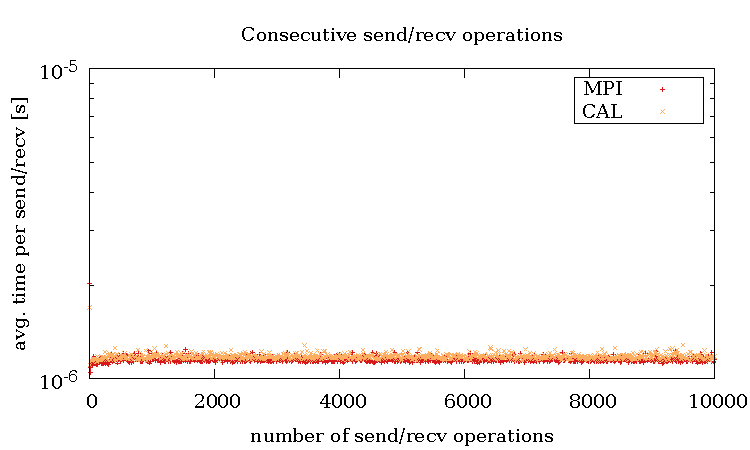
\includegraphics[width=\textwidth]{plots/50_nsend_cal_laser}
    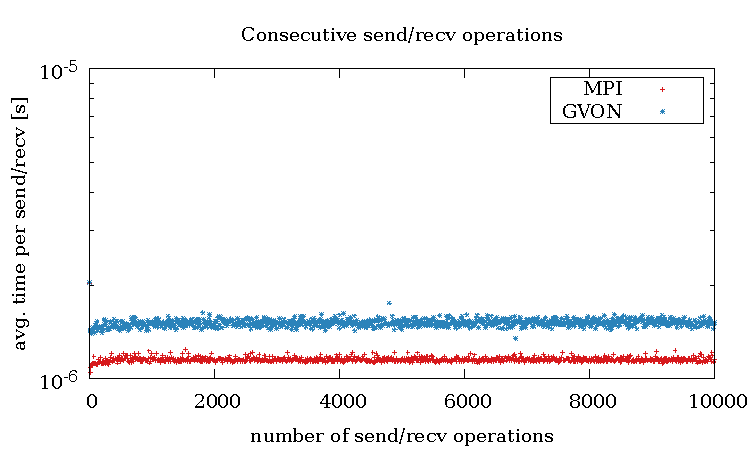
\includegraphics[width=\textwidth]{plots/50_nsend_gvon_laser}
    \end{minipage}%
  \begin{minipage}[t]{0.5\textwidth}
    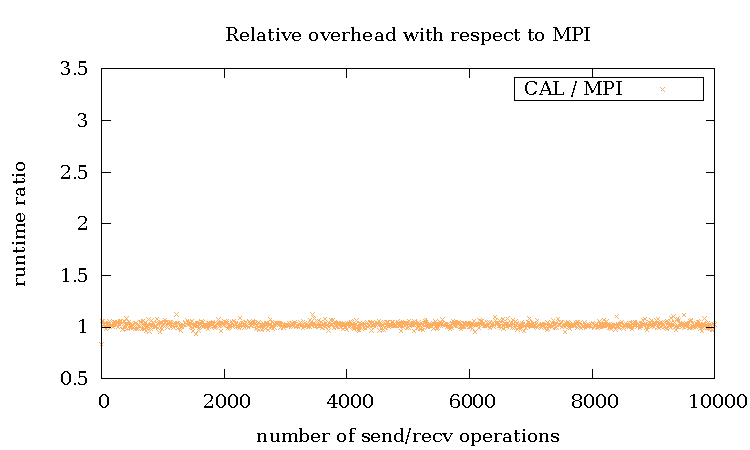
\includegraphics[width=\textwidth]{plots/50_nsend_overhead_cal}
    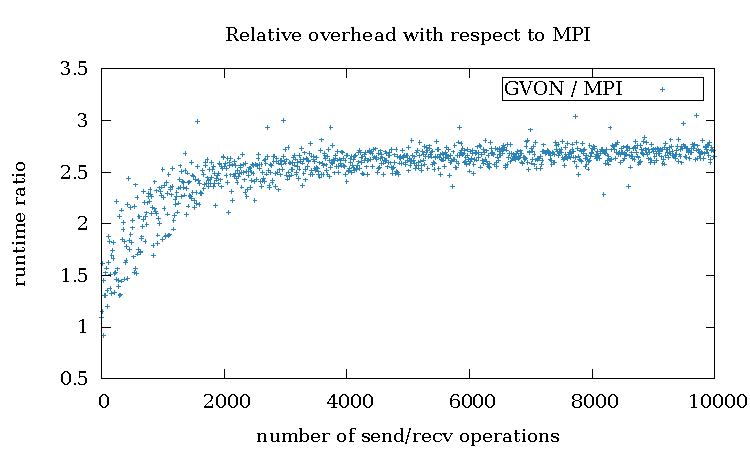
\includegraphics[width=\textwidth]{plots/50_nsend_overhead_gvon}
  \end{minipage}%
  \caption{Average run-time of a single send/recv operation and the
    according relative overhead of CAL and GVON with respect to
    MPI. The number of consecutive operations is increased from one to
    ten thousand by a step size of ten. }
  \label{fig:nsend_kepler}
\end{figure}

\noindent The relative overhead of the CAL and GVON stabilizes with
increasing number of send/recv operations.  The CAL adds a constant
average overhead of around two percent per send/recv operation with
respect to MPI through virtual address and context translations. The
GVON adds a constant average overhead of around thirty percent per
send/recv operation.  Since the communication topology of the GVON is
modeled by a graph, containing two nodes connected by a directed edge,
the constantly look up of this graph adds a constant overhead to each
send/recv operation.  Instead, the CAL and MPI are sending to and
receiving from fixed peer addresses without the need for a look up.
However, because the graph is not changing during the experiment, it
is sufficient to perform the graph look up only once. Experiments
performed with only one graph look up will be named GVON OGL. The one
look up variant should reduce the overhead to the similar level of
the CAL. Figure~\ref{fig:nsend_one_lookup_kepler} shows the results of
the experiment that only performs one look up per $n$ send/recv
operation.

\begin{figure}[H]
  \begin{minipage}[t]{0.5\textwidth} 
    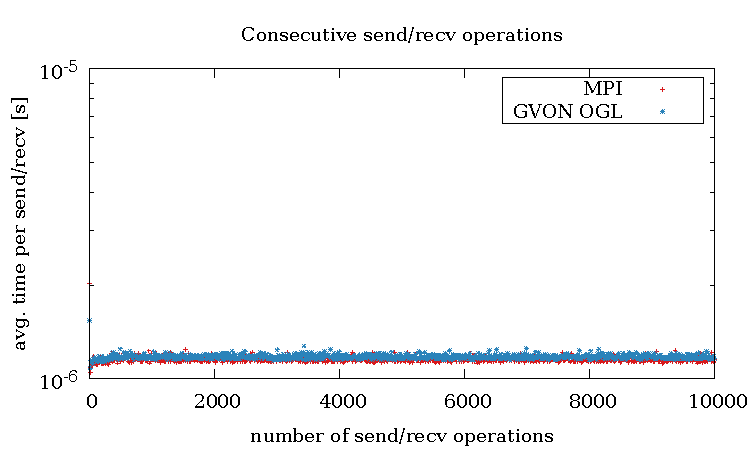
\includegraphics[width=\textwidth]{plots/50_nsend_one_lookup_laser}
  \end{minipage}%
  \begin{minipage}[t]{0.5\textwidth}
    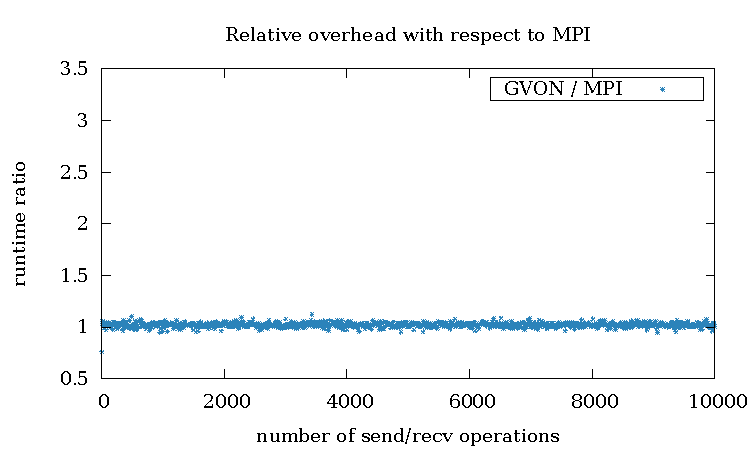
\includegraphics[width=\textwidth]{plots/50_nsend_one_lookup_overhead_gvon_laser}
  \end{minipage}%
  \caption{The amount of graph look ups is reduced to one look up for
    $n$ send/recv operations.  This reduces the GVON overhead to
    a similar level of the CAL.}
  \label{fig:nsend_one_lookup_kepler}
\end{figure}

\noindent Changing the experiment to a one look up variant, reduced
the GVON overhead to the same level of the CAL (around two
percent). Nevertheless, vertices and graphs need to be translated to
virtual addresses and contexts, such that, a small overhead with
respect to the CAL is still present. It shows that the graph
implementation needs to be optimized with regard to the look up of
incoming and outgoing edges in future work.

% Checked
\subsection*{Increase the Number of Elements per Send/Recv Operation $m$}
This experiment increases the number of elements $m$ per send/recv
operation from one to ten thousand by a step size of ten. A single
experiment obtains the average run-time over thousand operations.
This experiment is limited to execution on a single node. Thus, no
network latency is included in the
results. Figure~\ref{fig:nsize_kepler} shows the averaged run-time of
a send/recv operation for an increasing number element and the
run-time ration with respect to MPI.

\begin{figure}[H]
  \begin{minipage}[t]{0.5\textwidth}
    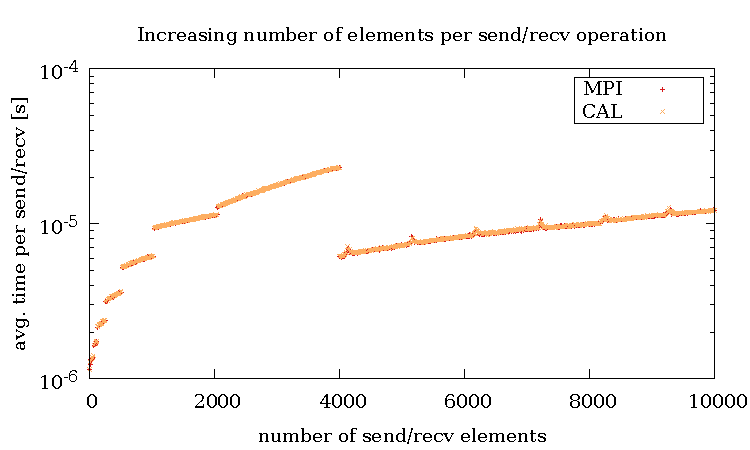
\includegraphics[width=\textwidth]{plots/50_nsize_cal_laser}
    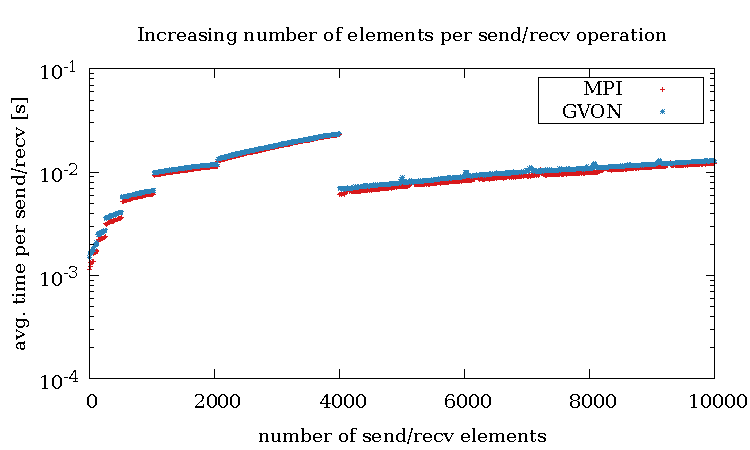
\includegraphics[width=\textwidth]{plots/50_nsize_gvon_laser}
    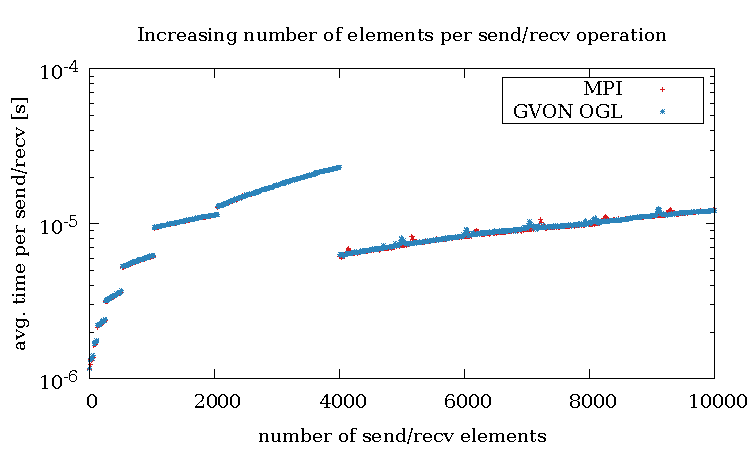
\includegraphics[width=\textwidth]{plots/50_nsize_one_lookup_gvon_laser}
  \end{minipage}%
  \begin{minipage}[t]{0.5\textwidth}
    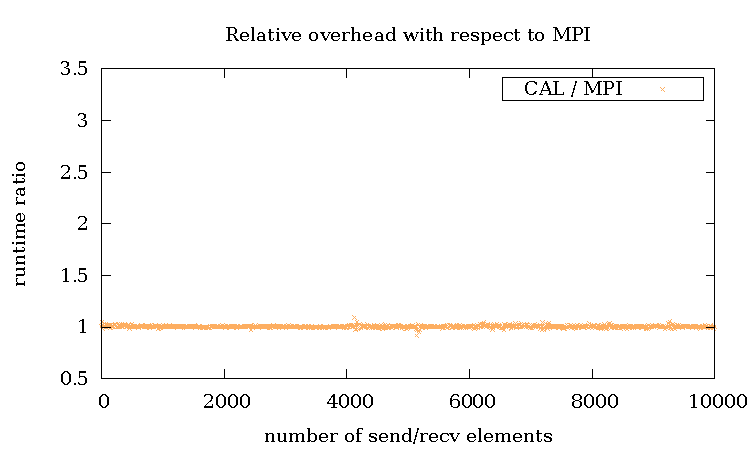
\includegraphics[width=\textwidth]{plots/50_nsize_overhead_cal_laser}
    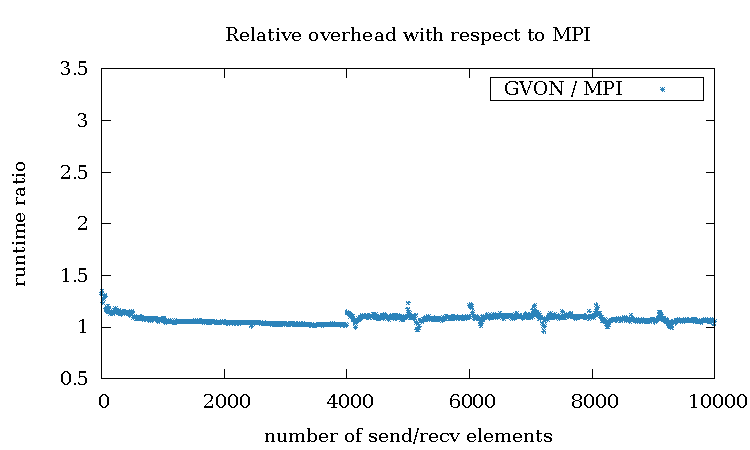
\includegraphics[width=\textwidth]{plots/50_nsize_overhead_gvon_laser}
    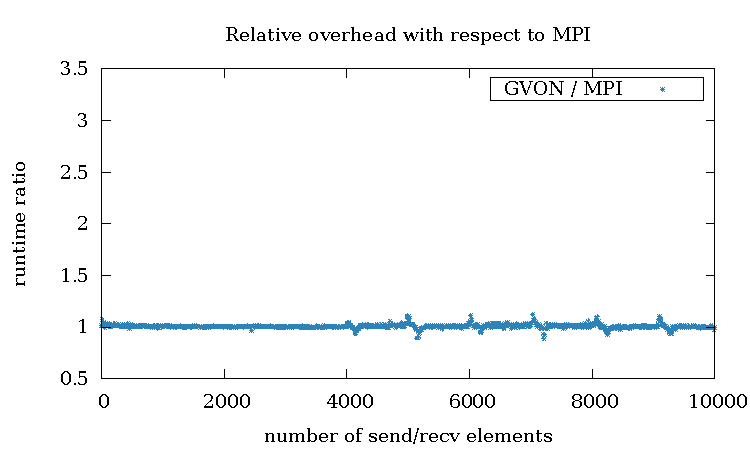
\includegraphics[width=\textwidth]{plots/50_nsize_one_lookup_overhead_gvon_laser}
  \end{minipage}%
  \caption{Increasing the number of elements per send/recv operations,
    reduces the relative overhead in respect to MPI.}
  \label{fig:nsize_kepler}
\end{figure}

\noindent With increasing number of elements per send/recv operations,
the run-time of CAL and GVON implementations converge with the
run-time of MPI implementation. The average overhead of the CAL is
negligible (less then one percent) and the average overhead of the
GVON is reduced to around seven percent per send/recv operation. The
last pair of Figures shows, that changing the GVON experiment to a one
graph look up variant drops the GVON run-time overhead to a negligible
level.

% Checked
\subsection*{Including Network}
The synthetic benchmark with increased number of elements per
send/recv operation mentioned above were performed only locally on a
single node.  Therefore, the run-time measurements were not influenced
by network latency.  This experiment setup is changed to a
configuration with two nodes, whereby the peers are not located on the
same node. It is expected, that the relative overhead of CAL and GVON
decreases even more in contrast to the previous experiments, while the
overall run-time will increase.  A setup of two laser nodes, each
hosting one peer, was selected.  Figure \ref{fig:nsend_network} shows
the average run-time of GVON and CAL with respect to MPI for
increasing send/recv operations including network latency.

\begin{figure}[H]
  \begin{minipage}[t]{0.5\textwidth}
    %% 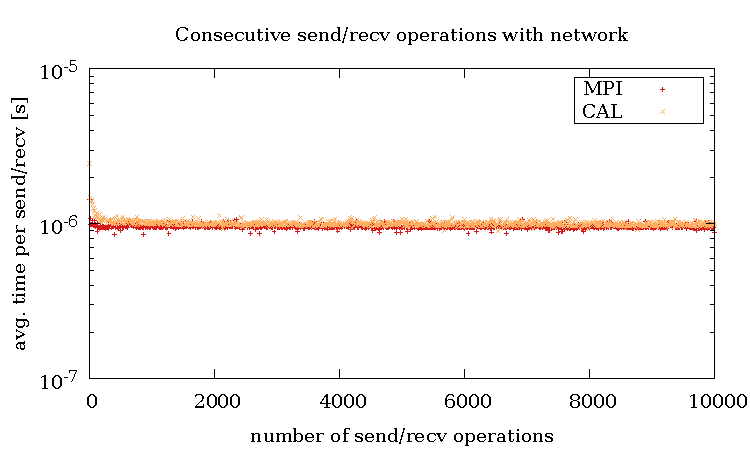
\includegraphics[width=\textwidth]{plots/50_nsend_network_cal_laser}
    %% 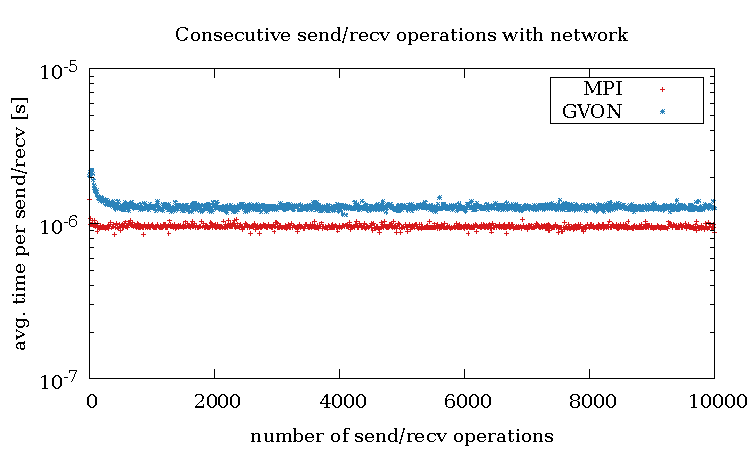
\includegraphics[width=\textwidth]{plots/50_nsend_network_gvon_laser}
    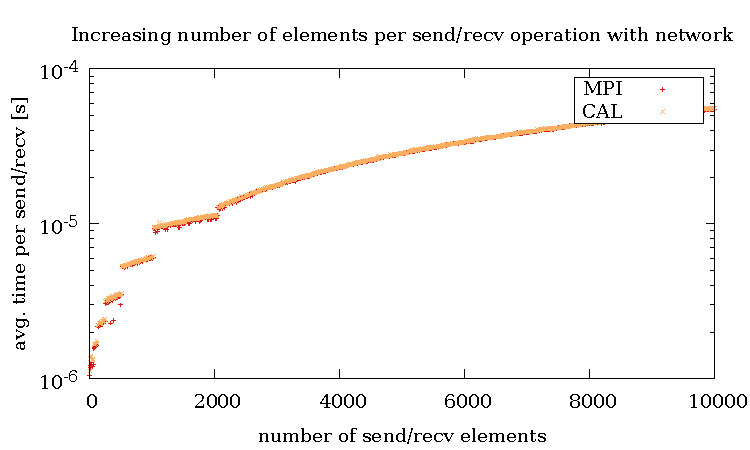
\includegraphics[width=\textwidth]{plots/50_nsize_network_cal_laser}
    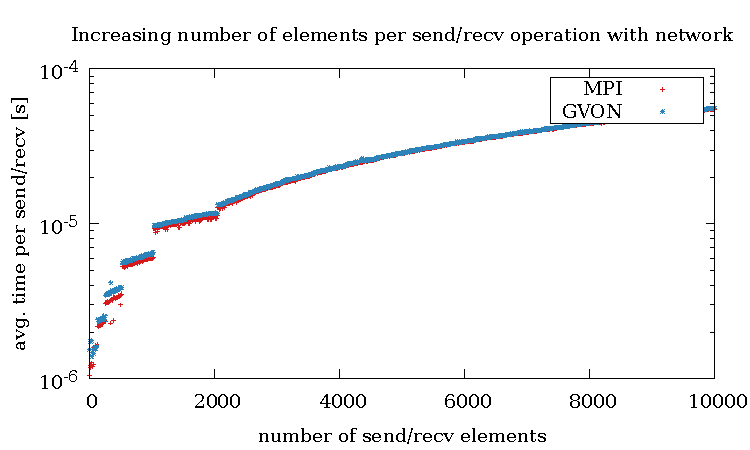
\includegraphics[width=\textwidth]{plots/50_nsize_network_gvon_laser}
    %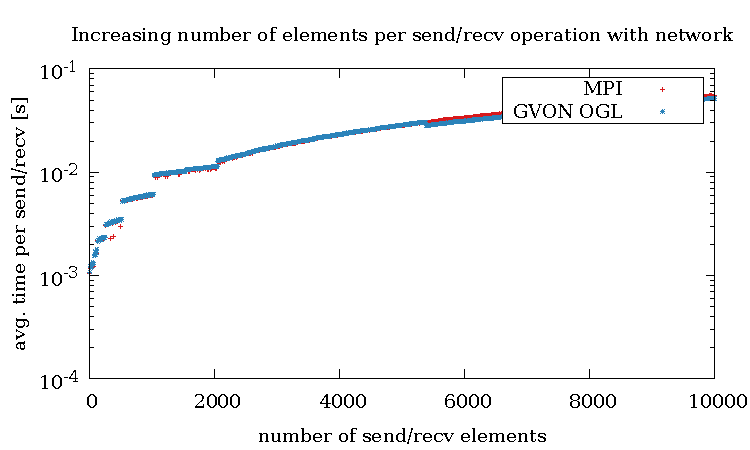
\includegraphics[width=\textwidth]{plots/50_nsize_one_lookup_network_gvon_laser}
  \end{minipage}%
  \begin{minipage}[t]{0.5\textwidth}
    %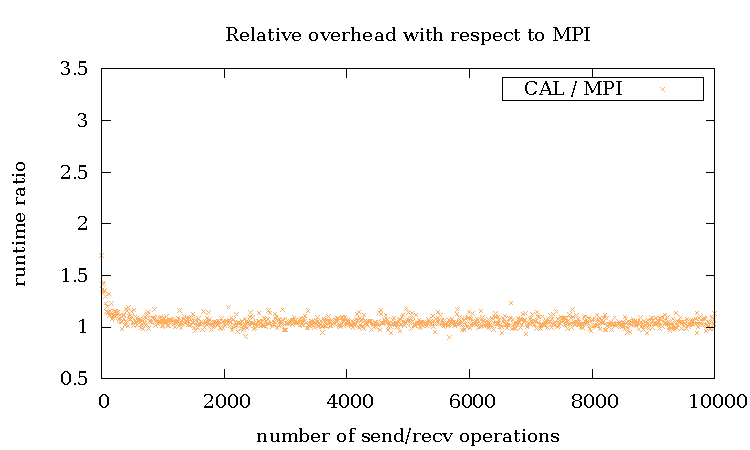
\includegraphics[width=\textwidth]{plots/50_nsend_network_overhead_cal_laser}
    %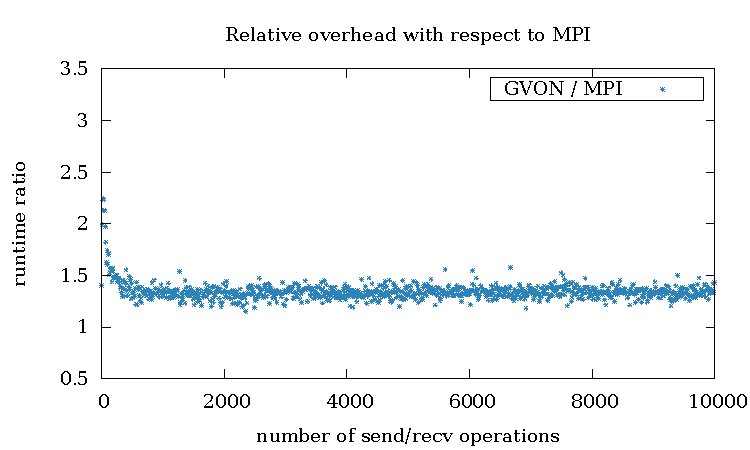
\includegraphics[width=\textwidth]{plots/50_nsend_network_overhead_gvon_laser}
    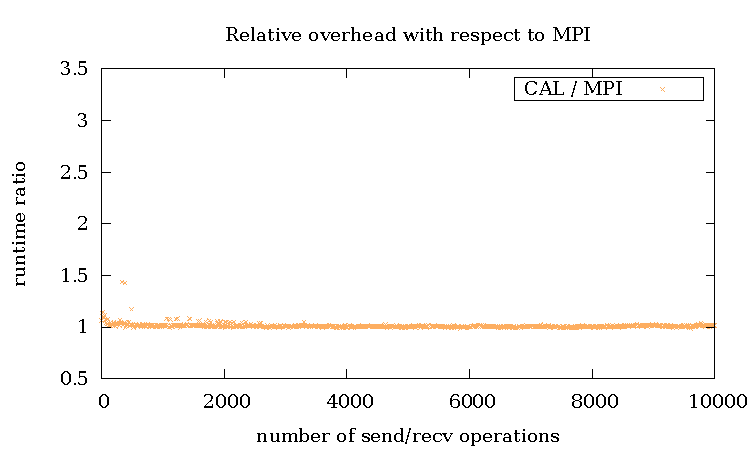
\includegraphics[width=\textwidth]{plots/50_nsize_network_overhead_cal_laser}
    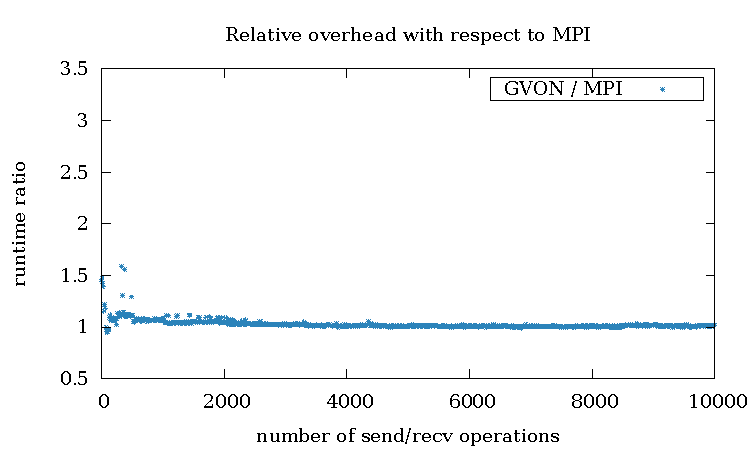
\includegraphics[width=\textwidth]{plots/50_nsize_network_overhead_gvon_laser}
    %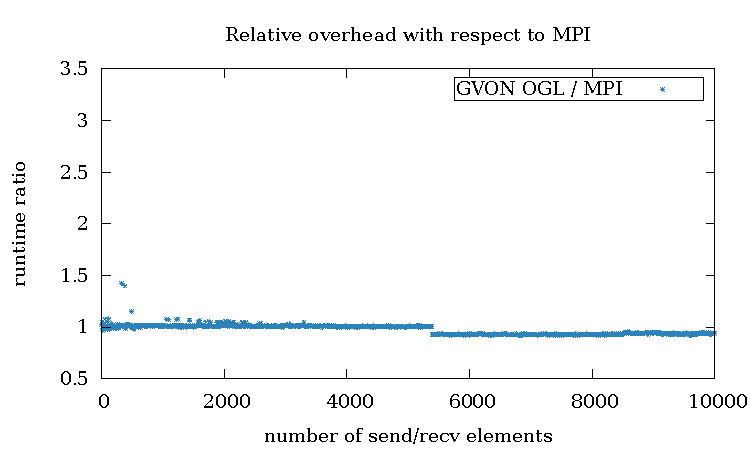
\includegraphics[width=\textwidth]{plots/50_nsize_one_lookup_network_overhead_gvon_laser}
  \end{minipage}%
  \caption{Increasing the number of elements per send/recv operations
    with the influence of network.}
  \label{fig:nsend_network}
\end{figure}

\noindent This experiment resembles more with a real world simulation,
because these simulation usually sends more than a single element per
communication operation and communicate over anetwork.  The CAL and
GVON overhead of these point-to-point operations is in an acceptable
range (a~few percent).  Therefore, the GVON can be considered for the
deployment in real world simulations.


%%%%%%%%%%%%%%%%%%%%%%%%%%%%%%%%%%%%%%%%%%%%%%%%%%%%%%%%%%%%%%%%%%%%%%%%%%%%%%%%
%                                                                              %
% SYNTHETIC COLLECTIVE BENCHMARK                                               %
%                                                                              %
%%%%%%%%%%%%%%%%%%%%%%%%%%%%%%%%%%%%%%%%%%%%%%%%%%%%%%%%%%%%%%%%%%%%%%%%%%%%%%%%
% Checked
\section{Synthetic Collective Benchmark}
This benchmark compares the run-time of MPI collectives with
equivalent collectives of the CAL and GVON.  To determine the run-time
for a single collective execution, the measurement is averaged over a
thousand executions.  Since, the overhead with respect to MPI should be
determined, only the gather and reduce collective were chosen for
comparison. Other collective operations behave in an analog
manner. These experiments will be executed on a setup with 8 laser
nodes, while the number of peers per nodes will be increased from one
CPU to a maximum of 64 CPUs.  This will lead to maximum number of 512
CPUs.

% Checked
\subsection*{Gather Collective}
This experiment evaluates the gather operation of MPI in comparison to
the CAL and GVON gather operations.  The GVON gather operation is first performed locally
for all hosted vertices of a host. Furthermore, a reordering of the
gather results in vertex index order is performed. An overhead with
respect to MPI is expected.  Figure \ref{fig:gather_laser} shows the
average run-time of a gather operation for increasing number of peers
including network latency.

\begin{figure}[H]
  \begin{minipage}[t]{0.5\textwidth}
    %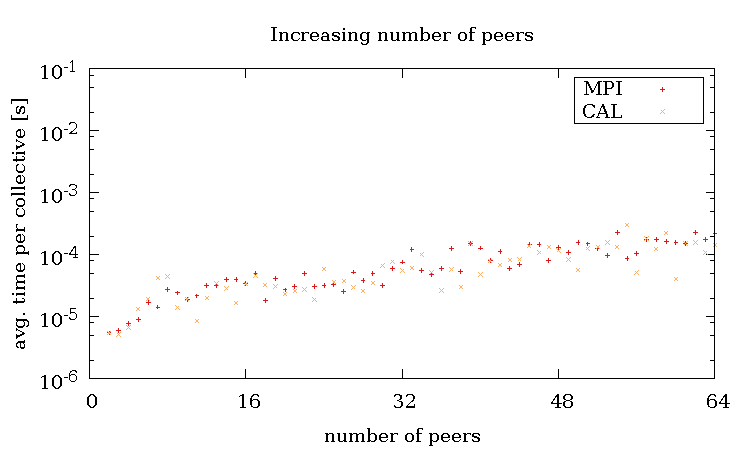
\includegraphics[width=\textwidth]{plots/50_collective_npeers_cal_laser}
    %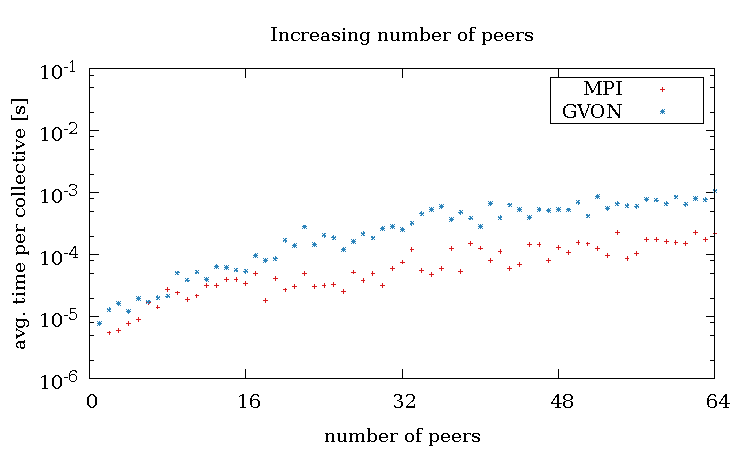
\includegraphics[width=\textwidth]{plots/50_collective_npeers_gvon_laser}
    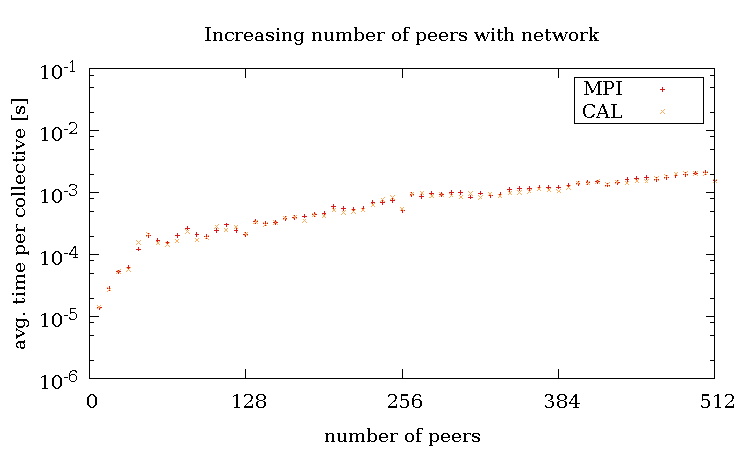
\includegraphics[width=\textwidth]{plots/50_collective_network_cal_laser}
    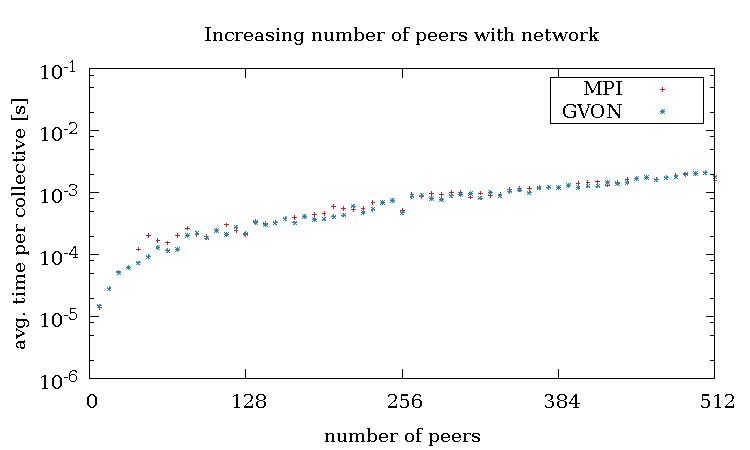
\includegraphics[width=\textwidth]{plots/50_collective_network_gvon_laser}
  \end{minipage}%
  \begin{minipage}[t]{0.5\textwidth}
    %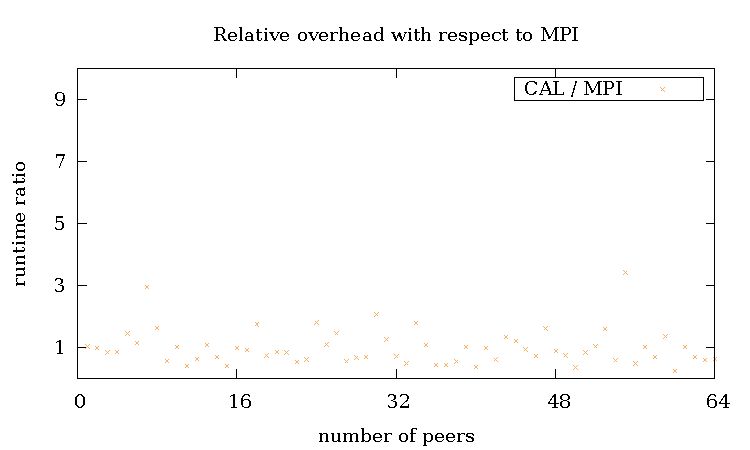
\includegraphics[width=\textwidth]{plots/50_collective_npeers_overhead_cal_laser}
    %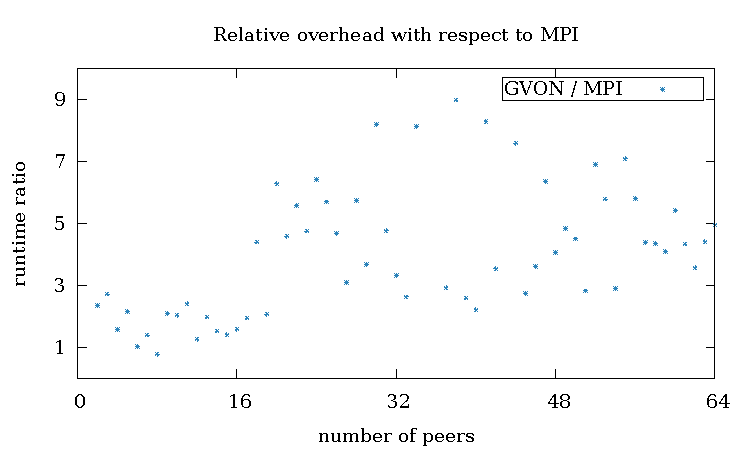
\includegraphics[width=\textwidth]{plots/50_collective_npeers_overhead_gvon_laser}
    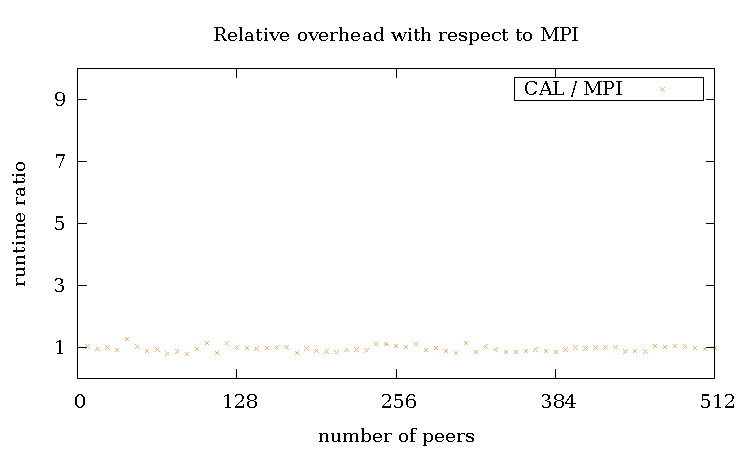
\includegraphics[width=\textwidth]{plots/50_collective_network_overhead_cal_laser}
    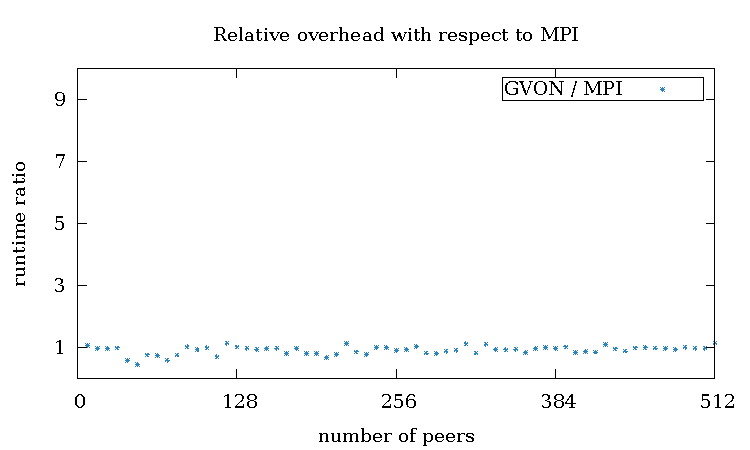
\includegraphics[width=\textwidth]{plots/50_collective_network_overhead_gvon_laser}
  \end{minipage}%
  \caption{ }
  \label{fig:gather_laser}
\end{figure}

\noindent Differently than expected, is the run-time overhead of the CAL and GVON
negligible or even not present. Collective operations of the GVON
do not require a look up of graph information. Thus, a source of
overhead mentioned in the previous benchmarks is not present on
this experiment.

% Checked
\subsection*{Reduce Collective}
This experiment evaluates the reduce operation of MPI in comparison to
the CAL and GVON reduce operations.  The reduce operation of the GVON
performs a local reduce first.  Figure \ref{fig:reduce_laser} shows
the average run-time of a reduce collective for increasing number of
peers with and without network.

\begin{figure}[H]
  \begin{minipage}[t]{0.5\textwidth}
    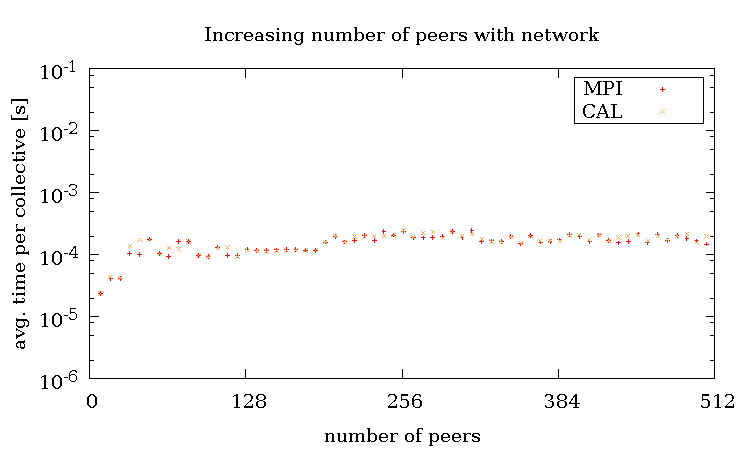
\includegraphics[width=\textwidth]{plots/50_reduce_network_cal_laser}
    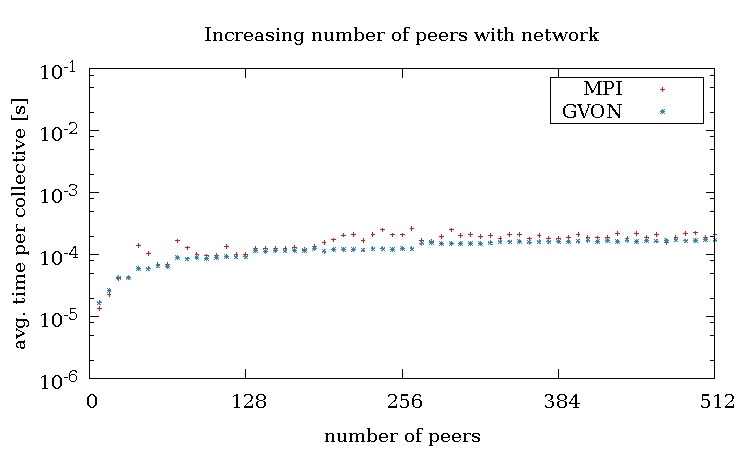
\includegraphics[width=\textwidth]{plots/50_reduce_network_gvon_laser}
  \end{minipage}%
  \begin{minipage}[t]{0.5\textwidth}
    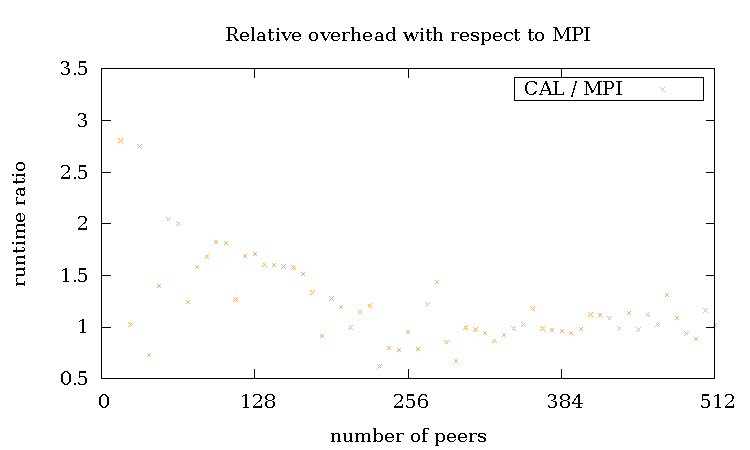
\includegraphics[width=\textwidth]{plots/50_reduce_network_overhead_cal_laser}
    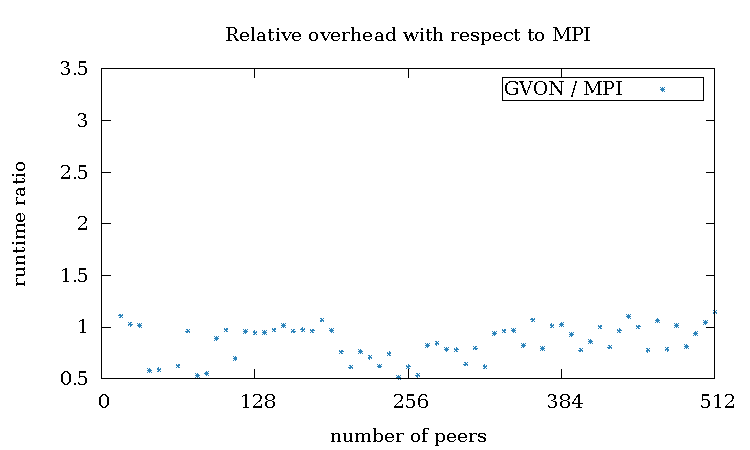
\includegraphics[width=\textwidth]{plots/50_reduce_network_overhead_gvon_laser}
  \end{minipage}%
  \caption{ }
  \label{fig:reduce_laser}
\end{figure}

\noindent This experiment behaves similar to the gather experiment with the
exception of some outliers. These outliers are normal in such a
network based environment and therefore no reason to complain about.


%%%%%%%%%%%%%%%%%%%%%%%%%%%%%%%%%%%%%%%%%%%%%%%%%%%%%%%%%%%%%%%%%%%%%%%%%%%%%%%%
%                                                                              %
% REAL WORLD SIMULATION BENCHMARK                                              %
%                                                                              %
%%%%%%%%%%%%%%%%%%%%%%%%%%%%%%%%%%%%%%%%%%%%%%%%%%%%%%%%%%%%%%%%%%%%%%%%%%%%%%%%
% Checked
\section{Real World Simulation Benchmark}
\label{sec:eval:real}
The previous benchmarks evaluated the developed system in a very
synthetic and unreal fashion. But, real world simulations perform
usually calculations in between their communication
operations. Furthermore, it is usual to overlap calculations by
non-blocking communication operations. Experiments evaluating the Game
of Life and N-body simulations were chosen as examples for such real
world simulations. These experiments compare the implementations on
top of the GVON from Section~\ref{sec:implementation} to equivalent
MPI implementations.  Equivalent refers to the same amount of
communication operations and that the same functions are used to
calculate or update the simulation states. A setup with 8 laser nodes
is used. The number of peers per node is incremented for each
measurement from one peer to a maximum of 64 peers. The peers are
equally distributed to the nodes.  Which leads to maximum number of
512 peers.


%%%%%%%%%%%%%%%%%%%%%%%%%%%%%%%%%%%%%%%%%%%%%%%%%%%%%%%%%%%%%%%%%%%%%%%%%%%%%%%%
%                                                                              %
% GAME OF LIFE BENCHMARK                                                       %
%                                                                              %
%%%%%%%%%%%%%%%%%%%%%%%%%%%%%%%%%%%%%%%%%%%%%%%%%%%%%%%%%%%%%%%%%%%%%%%%%%%%%%%%
% Checked
\subsection{Game of Life Benchmark}
This experiment compares the GVON implementation of the Game of Life
from Section~\ref{sec:impl:gol} with an equivalent MPI
implementation. The GoL domain is a rectangular field and the state of
every cell is calculated exclusively by one peer. The average run-time
for a time-step for an increasing number of cells is measured. The
run-time is measured with the influence of network latency.
Figure~\ref{fig:gol_laser} shows the average run-time of a time-step
dependent on the number of cells.

\begin{figure}[H]
  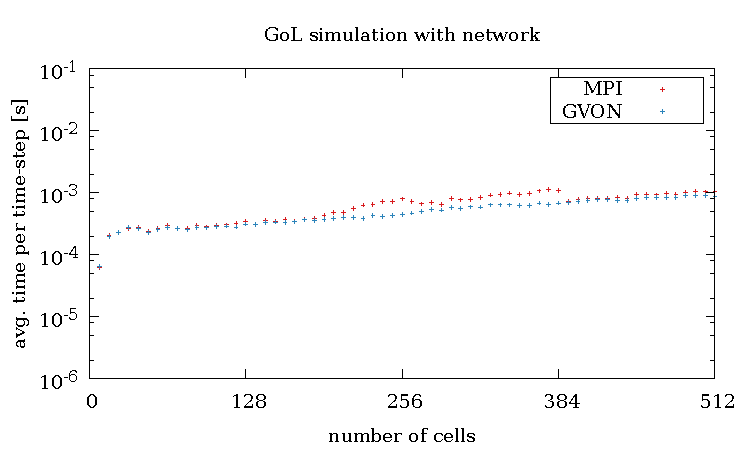
\includegraphics[width=\textwidth]{plots/50_gol_network_laser}
  \caption{Average run-time of GoL simulation for increasing number
    of cells.}
  \label{fig:gol_laser}
\end{figure}

\noindent The GVON implementation shows no overhead in comparison to
the MPI implementation. This behavior was expected, because
communication operations are overlapped with next state calculations.


%%%%%%%%%%%%%%%%%%%%%%%%%%%%%%%%%%%%%%%%%%%%%%%%%%%%%%%%%%%%%%%%%%%%%%%%%%%%%%%%
%                                                                              %
% N BODY BENCHMARK                                                             %
%                                                                              %
%%%%%%%%%%%%%%%%%%%%%%%%%%%%%%%%%%%%%%%%%%%%%%%%%%%%%%%%%%%%%%%%%%%%%%%%%%%%%%%%
% Checked
\subsection{N-Body Benchmark}
This benchmark evaluates the implemented N-body simulation increasing
number of bodies. It is compared an implementation based on MPI to an
implementation based on the GVON.  Thereby, each body is managed by a
peer. Therefore, the number of peers increases with the number of
bodies. Figure~\ref{fig:nbody_laser} shows the averaged run-time of a
time-step with dependence to the number of bodies.

\begin{figure}[H]
  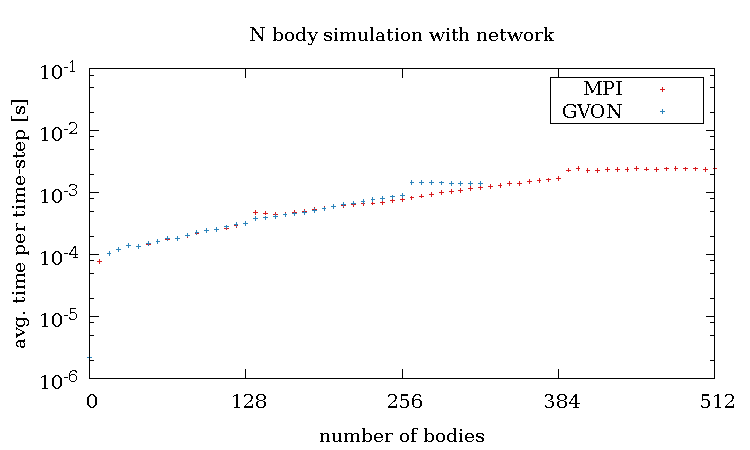
\includegraphics[width=\textwidth]{plots/50_nbody_network_laser}
  \caption{Average run-time of N-body simulation for increasing
    number of bodies. The simulation is executed with network.}
  \label{fig:nbody_laser}
\end{figure}

\noindent Analog to the GoL simulation shows this experiment no
overhead in comparison to the MPI implementation. Both real world
simulations have shown that the usage of the GVON communication
approach does not add overhead to the execution of communication
methods.

%%%%%%%%%%%%%%%%%%%%%%%%%%%%%%%%%%%%%%%%%%%%%%%%%%%%%%%%%%%%%%%%%%%%%%%%%%%%%%%%
%                                                                              %
% FLEXIBILITY BENCHMARK                                                        %
%                                                                              %
%%%%%%%%%%%%%%%%%%%%%%%%%%%%%%%%%%%%%%%%%%%%%%%%%%%%%%%%%%%%%%%%%%%%%%%%%%%%%%%%
\section{Flexibility Benchmark}

This benchmark analyzes the impact of redistribution of hosted
vertices to a varying set of hosts at run-time. A simulation based on the
GVON is executed by a number of hosts $h$. After a period of time steps
$t$, $h$ is varied.

The Peers are distributed equally over a set of laser nodes and
every peer hosts approximately the same number vertices.

\subsection{GoL Flexibility Benchmark}

The GoL simulation described in Section~\ref{sec:impl:gol} forms the
basis of this experiment.  The simulation is started with 256 peers
and the game field contains 8000 cells. The vertices of the modeled
GoL graph is distributed to the peers by a round robin algorithm.  The
number of hosts is decreased by one every ten time steps until the
number of hosts is equal to one. From this point the experiment
increases the number of hosts by one every ten time steps until the
number of peers is equal to 256. Figure~\ref{fig:gol_flexi_laser}
shows the average run-time of a single GoL time step whereby the
number of hosts are varied.

\begin{figure}[H]
  \includegraphics[width=\textwidth]{plots/50_gol_flexi_laser}
  \caption{Average time per time step with a varying number of
    hosts. First, the number of hosts is decreased from 256 to
    one. Second, the number of hosts is increased from one to 256.}
  \label{fig:gol_flexi_laser}
\end{figure}

\noindent Reducing the number of hosts means that the remaining hosts are
responsible for more hosted vertices. Therefore, the run-time should increase
with decreasing number of hosts.  But differently then expected, the
average run-time decreases with the decreasing number of hosts at the
beginning of the experiment. Therefore, less peers can also imply more
data locality which further implies a faster access to the state of
neighboring cells.

The average time per time step reaches its minimum at 64 hosts. This
point defines a distribution of vertices where the hosts are saturated
with vertices.  Decreasing the number of hosts even more only
increases the run-time of a time step. The run-time maximum is reached
when the whole simulation is calculated by a single host.  Increasing
the number of hosts from a single host back to 256 hosts shows
symmetrical behavior.


%%%%%%%%%%%%%%%%%%%%%%%%%%%%%%%%%%%%%%%%%%%%%%%%%%%%%%%%%%%%%%%%%%%%%%%%%%%%%%%%
%                                                                              %
% Summary                                                                      %
%                                                                              %
%%%%%%%%%%%%%%%%%%%%%%%%%%%%%%%%%%%%%%%%%%%%%%%%%%%%%%%%%%%%%%%%%%%%%%%%%%%%%%%%

\todo{Write Evaluation summary}

\cleardoublepage

%%% Local Variables:
%%% TeX-master: "diplom"
%%% End:
